%%%%%%%%%%%%%%%%%%%%%%%%%%%%%%%%%%%%%%%%%
% Arsclassica Article
% LaTeX Template
% Version 1.1 (10/6/14)
%
% This template has been downloaded from:
% http://www.LaTeXTemplates.com
%
% Original author:
% Lorenzo Pantieri (http://www.lorenzopantieri.net) with extensive modifications by:
% Vel (vel@latextemplates.com)
%
% License:
% CC BY-NC-SA 3.0 (http://creativecommons.org/licenses/by-nc-sa/3.0/)
%
%%%%%%%%%%%%%%%%%%%%%%%%%%%%%%%%%%%%%%%%%

%----------------------------------------------------------------------------------------
%	PACKAGES AND OTHER DOCUMENT CONFIGURATIONS
%----------------------------------------------------------------------------------------

\documentclass[
12pt, % Main document font size
a4paper, % Paper type, use 'letterpaper' for US Letter paper
oneside, % One page layout (no page indentation)
%twoside, % Two page layout (page indentation for binding and different headers)
headinclude,footinclude, % Extra spacing for the header and footer
BCOR5mm, % Binding correction
]{scrartcl}
%%%%%%%%%%%%%%%%%%%%%%%%%%%%%%%%%%%%%%%%%
% Arsclassica Article
% Structure Specification File
%
% This file has been downloaded from:
% http://www.LaTeXTemplates.com
%
% Original author:
% Lorenzo Pantieri (http://www.lorenzopantieri.net) with extensive modifications by:
% Vel (vel@latextemplates.com)
%
% License:
% CC BY-NC-SA 3.0 (http://creativecommons.org/licenses/by-nc-sa/3.0/)
%
%%%%%%%%%%%%%%%%%%%%%%%%%%%%%%%%%%%%%%%%%

%----------------------------------------------------------------------------------------
%	REQUIRED PACKAGES
%----------------------------------------------------------------------------------------

\usepackage[
nochapters, % Turn off chapters since this is an article        
beramono, % Use the Bera Mono font for monospaced text (\texttt)
eulermath,% Use the Euler font for mathematics
pdfspacing, % Makes use of pdftex’ letter spacing capabilities via the microtype package
dottedtoc % Dotted lines leading to the page numbers in the table of contents
]{classicthesis} % The layout is based on the Classic Thesis style

\usepackage{arsclassica} % Modifies the Classic Thesis package

\usepackage[T1]{fontenc} % Use 8-bit encoding that has 256 glyphs

\usepackage[utf8]{inputenc} % Required for including letters with accents

\usepackage{graphicx} % Required for including images
\graphicspath{{Figures/}} % Set the default folder for images

\usepackage{enumitem} % Required for manipulating the whitespace between and within lists

\usepackage{lipsum} % Used for inserting dummy 'Lorem ipsum' text into the template

\usepackage{subfig} % Required for creating figures with multiple parts (subfigures)

\usepackage{amsmath,amssymb,amsthm} % For including math equations, theorems, symbols, etc

\usepackage{varioref} % More descriptive referencing

%----------------------------------------------------------------------------------------
%	THEOREM STYLES
%---------------------------------------------------------------------------------------

\theoremstyle{definition} % Define theorem styles here based on the definition style (used for definitions and examples)
\newtheorem{definition}{Definition}

\theoremstyle{plain} % Define theorem styles here based on the plain style (used for theorems, lemmas, propositions)
\newtheorem{theorem}{Theorem}

\theoremstyle{remark} % Define theorem styles here based on the remark style (used for remarks and notes)

%----------------------------------------------------------------------------------------
%	HYPERLINKS
%---------------------------------------------------------------------------------------

\hypersetup{
%draft, % Uncomment to remove all links (useful for printing in black and white)
colorlinks=true, breaklinks=true, bookmarks=true,bookmarksnumbered,
urlcolor=webbrown, citecolor=webgreen, % Link colors
pdftitle={}, % PDF title
pdfauthor={\textcopyright}, % PDF Author
pdfsubject={}, % PDF Subject
pdfkeywords={}, % PDF Keywords
pdfcreator={pdfLaTeX}, % PDF Creator
pdfproducer={LaTeX with hyperref and ClassicThesis} % PDF producer
} % Include the structure.tex file which specified the document structure and layout
\usepackage{fancybox}
\usepackage{listings}
\usepackage{tikz}


\hyphenation{Fortran hyphenation} % Specify custom hyphenation points in words with dashes where you would like hyphenation to occur, or alternatively, don't put any dashes in a word to stop hyphenation altogether


%----------------------------------------------------------------------------------------
%	TITLE AND AUTHOR(S)
%----------------------------------------------------------------------------------------

\title{\normalfont\spacedallcaps{F\MakeLowercase{u}LBLINK\MakeLowercase{y}} \\
\normalfont\spacedallcaps{User Guide}}% The article title


%----------------------------------------------------------------------------------------

\begin{document}

%----------------------------------------------------------------------------------------
%	HEADERS
%----------------------------------------------------------------------------------------
\newcommand{\titlebox}[2]{
\begin{tikzpicture}
\node[draw,thick,inner sep=6mm] (titlebox) {#2};
\node[fill=white] (Title) at (titlebox.north) {\bfseries \large #1};
\end{tikzpicture}
}
\renewcommand{\sectionmark}[1]{\markright{\spacedlowsmallcaps{#1}}} % The header for all pages (oneside) or for even pages (twoside)

%\lehead{\mbox{\llap{\small\thepage\kern1em\{halfgray} \vline}\color{halfgray}\hspace{0.5em}\rightmark\hfil} % The header style
\newcommand{\titledframe}[2]{%
       \boxput*(0,1){\psframebox*{#1}}%
         {\psframebox[framesep=12pt]{#2}}}
         
\pagestyle{scrheadings} % Enable the headers specified in this block


%----------------------------------------------------------------------------------------
%	TABLE OF  CONTENTS & LISTS OF FIGURES AND TABLES
%----------------------------------------------------------------------------------------

\maketitle % Print the title/author/date block

\setcounter{tocdepth}{2} % Set the depth of the table of contents to show sections and subsections only

\tableofcontents % Print the table of contents



%----------------------------------------------------------------------------------------
%	ABSTRACT
%----------------------------------------------------------------------------------------

\section*{Abstract} % This section will not appear in the table of contents due to the star (\section*)
This document provides general information about using the FuLBLINKy software. FuLBLINKy is a visualization tool, created specifically for Computational Fluid Dynamics simulations, with particular focus on Lattice Boltzmann methods.



%----------------------------------------------------------------------------------------

\newpage % Start the article content on the second page, remove this if you have a longer abstract that goes onto the second page

%----------------------------------------------------------------------------------------
%	INTRODUCTION
%----------------------------------------------------------------------------------------

\section{Preparing your computer}
\subsection{Technical requirements}
Before installing FuLBLINKy, please make sure that the following software is installed on your machine:
\begin{itemize}
\item GLFW3 (\url{http://www.glfw.org/})
\item GLM (\url{http://glm.g-truc.net/0.9.6/index.html})
\item CEGUI 0.8+ (\url{http://cegui.org.uk/})
\item GTK 3.0+
\item A graphics driver compatible with OpenGL 3.3+
\end{itemize}


\subsection{Installation of FuLBLINKy}
If everything went well with the above steps, you should now have everything you need to build the project. Just make sure your \texttt{LD\_LIBRARY\_PATH} points to the location the GLFW and CEGUI libs were installed to (\texttt{/usr/local/lib} by default) and run \texttt{make} from the project directory. 

Once all software is installed, run the following command from the terminal in corresponding folder: \texttt{./fluid-vis}. This should open the FuLBLINKy user interface.
%\begin{lstlisting}[ caption = {Starting the program}, label={listing1}, numbers = left,language = {Promela}]
%./fluid-vis
%\end{lstlisting}

%----------------------------------------------------------------------------------------
%	GETTING STARTED
%----------------------------------------------------------------------------------------

\section{Getting started with FuLBLINKy}

FuLBLINKy provides two main options:
\begin{itemize}
\item Flow visualization from a \textit{.vtk} file;
\item Live visualization of a fluid flow simulation on arbitrary geometries using the Lattice Boltzmann method.
\end{itemize}
\begin{figure}
 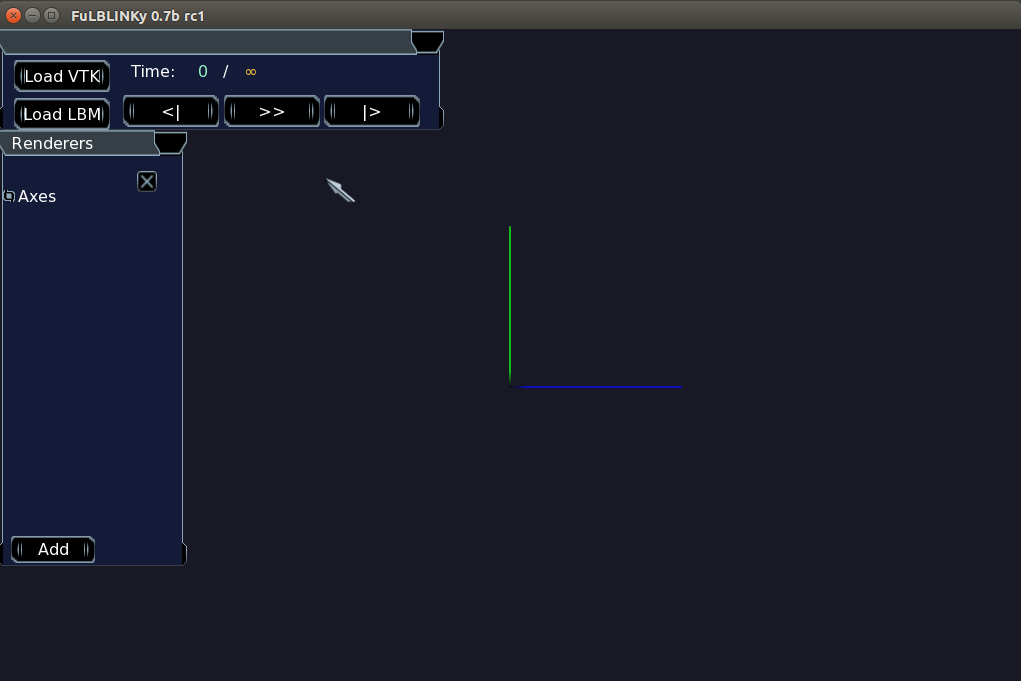
\includegraphics[width=0.8\textwidth]{fullblinky_start.png}
   \caption{Main window}
   \label{fig:fullblinky start}
\end{figure}

For the visualization of the flow from a given \textit{.vtk} file, press \textbf{"Load VTK"} button in the left upper corner of the screen (see fig. \ref{fig:fullblinky start}) and choose the appropriate input file. FuLBLINKy automatically detects files in the directory that are a part of the result sequence of the simulation. To navigate through the time steps use \textit{<|} (previous timestep) and \textit{|>} (next timestep) buttons. Use the \textit{>>} button for a continuous, forward-in-time visualization of a sequence of result files.

In order to run live LBM simulation, press \textbf{"Load LBM"} button in the left upper corner of the screen and choose an appropriate input file. Sample input files can be found here: \textit{ /lbsim/inputFiles}.

FuLBLINKy also supports standard camera features such as zoom in/zoom out and pan. Use mouse scroll to zoom in/out. For panning, press and hold the right mouse button and drag to adjust the image position.


\section{Data Visualization Options}
FuLBLINKy provides several standard data visualization options: Point data, vector-glyphs, line-glyphs, streamlines. In addition, FuLBLINKy also allows visualization of probability density values for the live LBM solver - a handy feature for debugging nasty LBM errors. 
\begin{figure}
 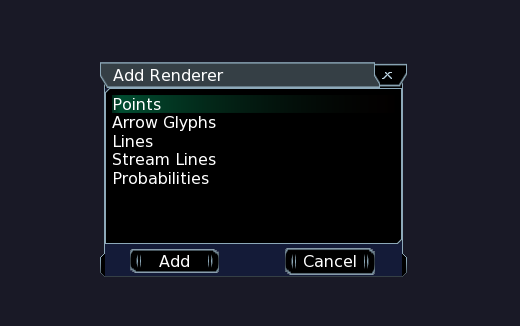
\includegraphics[width=0.8\textwidth]{addrenderer.png}
   \caption{Add renderer window}
   \label{fig:addrenderer}
\end{figure}

\subsection{Points}
To enable grid points colored according to the velocity values or density values:
\begin{itemize}
\item Press the button \textbf{Add}
\item Choose \textbf{Points} and press \textbf{Add} again (see fig. \ref{fig:addrenderer});
\item In the "Renderers" window under the appeared field \textbf{"Points"} choose the field you want to visualize from drop-down menu (see fig. \ref{fig:points}).
\end{itemize}
\begin{figure}
 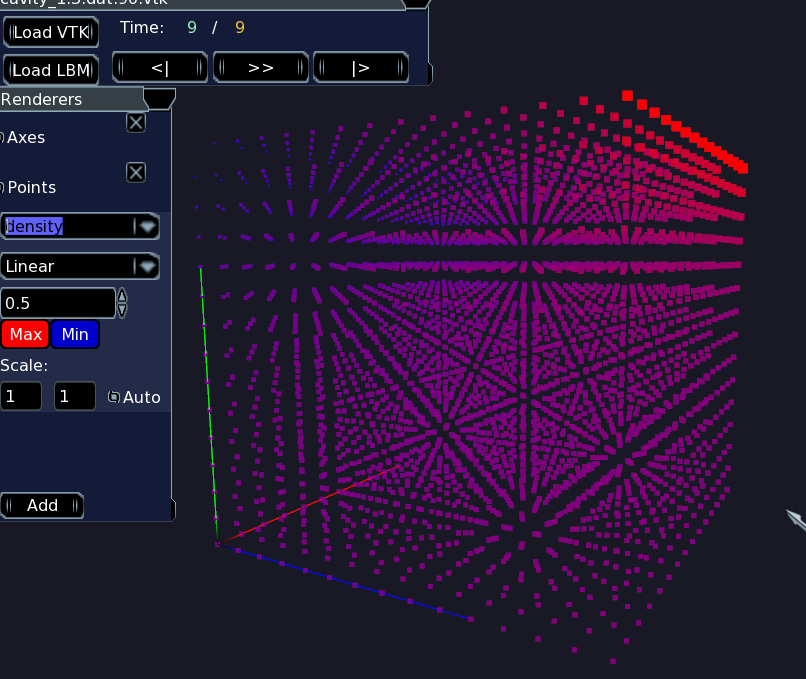
\includegraphics[width=0.8\textwidth]{density_points.png}
   \caption{Points renderer}
   \label{fig:points}
\end{figure}

\subsection{Glyphs}
To be able to see glyphs to the velocity (or other) values or density values:
\begin{itemize}
\item Press the button \textbf{Add}
\item Choose \textbf{Glyphs} and press \textbf{Add} again.
\item In the "Renderers" window under the appeared field \textbf{"Glyphs"} choose the field you want to visualize from drop-down menu (see fig. \ref{fig:glyphs}).
\end{itemize}
\begin{figure}
 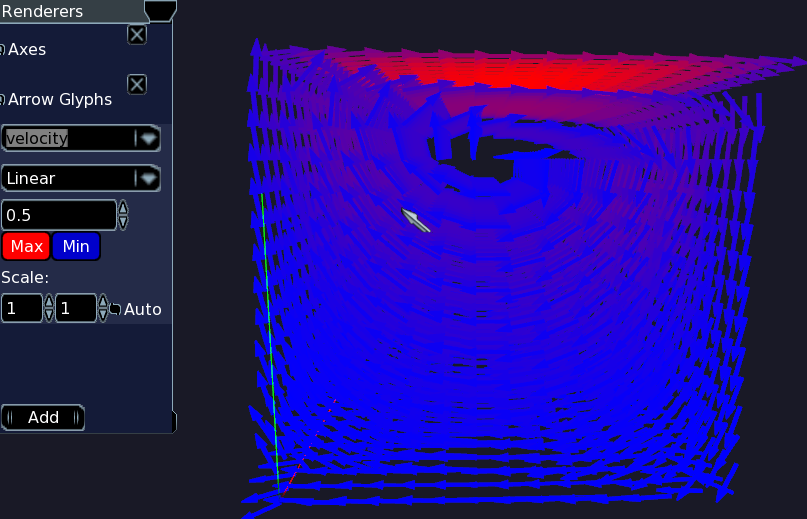
\includegraphics[width=0.8\textwidth]{glyphs.png}
   \caption{Glyphs renderer}
   \label{fig:glyphs}
\end{figure}

\subsection{Lines}
Analogical to Glyphs, but without specifying directions.

\subsection{Streamlines}
Streamlines are initiated as uniformly distributed points on a line source. To visualize streamlines (see fig. \ref{fig:streamlines}) from a line source:
\begin{itemize}
\item Press the button \textbf{Add}
\item Choose \textbf{Streamlines} and press \textbf{Add} again.
\item Enter the coordinates of start and end points of the line source in corresponding fields
\item Enter number of points on a line, which are to be used as a starting points for streamline
\item Enter maximum length of streamlines
\end{itemize}
To change thickness of streamlines uncheck \textbf{Auto} checkbox and enter the value in a field \textbf{Scale}.
\begin{figure}
 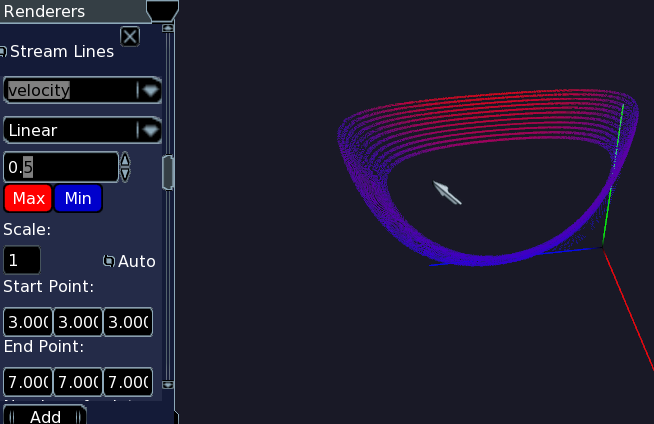
\includegraphics[width=0.8\textwidth]{streamlines.png}
   \caption{Streamline renderer}
   \label{fig:streamlines}
\end{figure}

\subsection{Probability distributions (LBM only)}
\begin{figure}[h]
 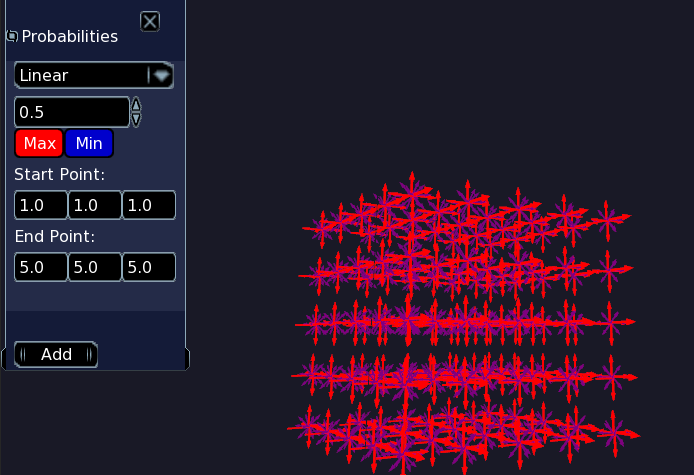
\includegraphics[width=0.8\textwidth]{probabilities.png}
 \caption{Probability distributions in lattice directions}
 \label{fig:probabilities}
\end{figure}
To visualize probability distributions in lattice directions (see fig. \ref{fig:probabilities}) (currently D3Q19 is used):
\begin{itemize}
\item Press the button \textbf{Add}.
\item Choose \textbf{Probabilities} and press \textbf{Add} again.
\item Enter the range for $x, y$ and $z$ coordinates points to be visualized.
\end{itemize}
Arrows are colored according to the relative probability magnitude. 




\section{Data Analysis Features}
In the current version of FuLBLINKy, several scaling options are provided to enable the user to highlight particular features of their flow results.

\subsection{Color Scaling}
The following scaling options are available for all visualization features:
\begin{itemize}
\item To change color scaling, pick one of the three options in the second drop-down menu:
\begin{itemize}
\item Linear
\item Smooth
\item Exponential
\end{itemize}
\item To set minimum and maximum values for color scaling use \textbf{min} and \textbf{max} color pickers.\\
\end{itemize}

\subsection{Size Scaling}
To change length scaling of the glyphs, uncheck \textbf{Auto} checkbox in the right lower corner of the \textit{renderers -> Points} window and enter an appropriate range in corresponding fields.

\end{document}
